\chapter{Avaliação Experimental}
\label{cap:experimentacao}

A avaliação foi sobre o Interceptador Hermes versão \gls{HTTP} e as aplicações: HttpLogClient e HttpLogServer. O HttpLogClient é um gerador de carga escrito em Python e tem a função de estressar o servidor da aplicação, enviando requisições HTTP. O HttpLogClient tem os seguintes parâmetros:

\begin{itemize}
\item \textit{address} do tipo \textit{TEXT}: define endereço do servidor;
\item \textit{port} do tipo \textit{INTEGER}: define porta do servidor;
\item \textit{bytes\_size} do tipo \textit{INTEGER}: define o tamanho da carga útil em número de bytes;
\item \textit{read\_rate} do tipo \textit{INTEGER}: define a taxa de leitura de 0 a 100 por cento;
\item \textit{n\_processes} do tipo \textit{INTEGER}: define número de processos do cliente;
\item \textit{thinking\_time} do tipo \textit{FLOAT}: define o tempo de reflexão entre as solicitações;
\item \textit{duration} do tipo \textit{FLOAT}: define a duração em segundos;
\end{itemize}

O HttpLogServer faz duas operações: \textit{get\_line(number)} (\textit{GET}) e \textit{append\_line(n-bytes-string)} (\textit{POST}). Estas funções são acionadas por requisições HTTP que podem ser realizadas pelos geradores de carga. Para acionar a função \textit{get\_line} basta enviar uma requisição \textit{GET} para \textit{/line/<number>}. Para acionar a função \textit{append\_line} basta enviar uma requisição \textit{POST} para \textit{/insert body: "128-byte-string"}. O \textit{HttpLogServer} tem os seguintes parâmetros:

\begin{itemize}
\item \textit{address} do tipo \textit{TEXT}: define endereço do servidor;
\item \textit{port} do tipo \textit{INTEGER}: define porta do servidor;
\end{itemize}

A função \textit{append\_line(n-byte-string)} é acionada por requisição \textit{POST} para \textit{/insert}, onde o corpo da mensagem é o conteúdo de uma \textit{string} de caracteres \gls{ASCII}, aleatória, e de tamanho parametrizável.
Em um primeiro momento foi necessário avaliar se os dados replicados corretamente, depois que foi visto que os \textit{logs} estavam sendo replicados, então começaram os experimentos de Latência (em nanosegundos) e, Vazão (número de requisições por segundo).

A avaliação se deu por examinar os dados brutos, para entender o comportamento do sistema perante algumas poucas cargas. A medida que se foi possível entender como aplicar cargas, foram feitos melhoramentos sobre os códigos do \textit{HttpLogServer} e \textit{HttpLogClient}.

Por exemplo o uso de \textit{Threads} em Python estava impedindo que os experimentos gerassem dados plausíveis, pois em Python não há concorrência real de \textit{Threads}. No entanto, o uso de Processos se apresentou como uma solução alternativa ao uso de \textit{Threads}.

\section{Medições}

\begin{figure}[htb!]
\centering
\caption{Esquematização de como e onde foram feitas as medições}
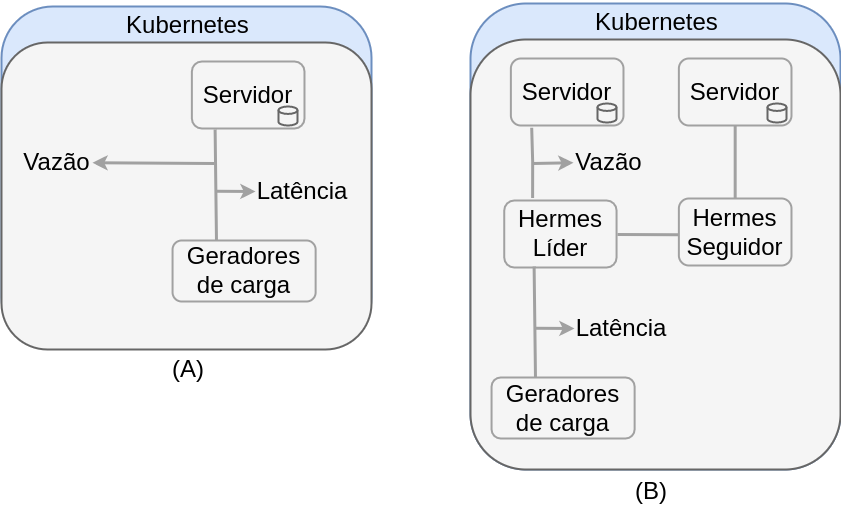
\includegraphics[width=0.8\linewidth]{figures/medicoes-configs.drawio.png}
{\flushleft Fonte - Própria.}
\label{fig:experimento-medicoes}
\end{figure}

A Figura \ref{fig:experimento-medicoes} ilustra em (A) que se trata de medições em um sistema sem replicação e em (B) que se trata de medições em um sistema replicado. Em (B), as entidades com nome \textit{Hermes Seguidor} representam 2 replicações, totalizando 3 réplicas juntamente com o Hermes Líder. A medição da vazão foi realizada como sendo a quantidade de requisições atendidas a cada segundo. A medição da latência foi feita como sendo o quanto tempo demora para executar uma requisição \gls{HTTP} e obter o retorno. As setas na figura (A) e (B) buscam mostrar onde o fluxo de informação foi capturado. Em (A) e (B) as latências são registradas no programa gerador de carga. Finalmente, em (A) e (B) as vazões são registradas no programa servidor sendo replicado.

\section{Ambiente de experimentação}

O ambiente de experimentação foi a plataforma Emulab\footnote{Emulab: \url{http://docs.emulab.net/}} \cite{emulab-10.1145/844128.844152}. Nesta plataforma foram alocadas 3 máquinas para os servidores de ordenação de mensagens e 2 máquinas para os geradores de carga. A máquina usada para os experimentos foi a d710. A especificações são as seguintes: marca Dell Poweredge R710, processador 2.4 GHz 64-bit Quad Core Xeon E5530 "Nehalem", cache de 8 MB L3, memória de 12 GB 1066 MHz DDR2 RAM (6 módulos de 2GB), discos rígidos de 500GB e 250GB 7200 rpm SATA.

% \begin{table}[htb!]
% \centering
% \caption{Máquinas usadas nos experimentos}
% \begin{tabular}{c|c|c|c|c}
% \textbf{Nome} & \textbf{Cores} & \textbf{Marca} & \textbf{Memória} & \textbf{Arquitetura} \\
% d430 & 8 & E5-2630v3 & 65536 & x86 64-bit \\
% d710 & 4 & Intel Quad Core Xeon E5530 & 12288 & x86 64-bit \\
% pc3000 & 1 & Xeon & 2048 & x86 64-bit \\
% \end{tabular}
% {\flushleft Fonte - Emulab}
% \label{tab:machines-emulab}
% \end{table}

\begin{figure}[htb!]
\centering
\caption{Esquematização dos nodos do Emulab}
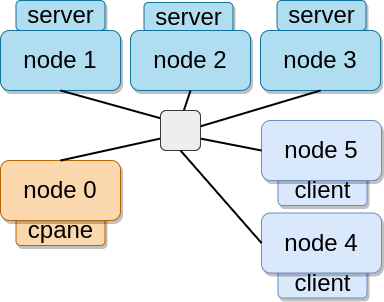
\includegraphics[width=0.45\linewidth]{figures/nodes.drawio.png}
{\flushleft Fonte - Própria.}
\label{fig:emulab-nodes}
\end{figure}

\pagebreak

A Figura \ref{fig:emulab-nodes} representa a configuração de nodos utilizada. A configuração apresentada mostra que foi pensado em deixar os servidores isolados, reduzindo ruídos. Alguns passos podem ser realizados para implantar um \textit{cluster} Kubernetes pronto para experimentação:

\begin{itemize}
\item É preciso instalar o Ansible\footnote{Ansible - \url{https://www.ansible.com/}} localmente.
\item Criar um experimento no Emulab e copiar os \textit{hosts}.
\item (Opcional) Listar os hosts no arquivo \textit{ansible/known\_hosts}.
\item (Opcional) Usar o \textit{script} \textit{scripts/ssh\_hosts.sh} para adicionar as chaves ssh. O script busca as interfaces de IP privada que serão usadas no passo do Kube Flannel. O script vai imprimir no terminal as interfaces e os IPs. Para configurar o Kube Flannel é necessário pegar apenas os IPs privados. IPs começando com \textsc{10.} são exemplos de IPs privados.
\item Configurar os \textit{hosts} do Emulab, em \textit{ansible/hosts}.
\item Configurar \textit{ansible\_user}, em \textit{ansible/hosts}.
\item Configurar o \textit{kubernetes/kube\_flannel.yaml} com os nomes das interfaces de rede privada que foram obtidas no passo anterior. Procurar por \textsc{--iface} no arquivo \textit{kubernetes/kube\_flannel.yaml}.
\item Executar o \textit{script} \textit{scripts/setup-emulab-cluster.sh}, para poder configurar o \textit{cluster} Kubernetes no Emulab. É preciso passar parâmetros para o script poder executar corretamente. Deve ser passado: caminho diretório Ansible; caminho diretório Kubernetes; nome do experimento no Emulab; nome do grupo no Emulab e a quantidade de servidores do tipo \textit{role=server}.
\item Instale o \textit{Kubectl} localmente, para poder executar os arquivos de descrição do Kubernetes.
\end{itemize}

\section{Caracterização da carga de trabalho utilizada}

O procedimento para capturar um conjunto de combinações de número de clientes e número de processos por cliente foi através de uma progressão sucessiva de carga, aumento do número de processos, variando o número de máquinas entre 1 e 2. Assim foi possível entender como a aplicação sem replicação estava se comportando com o aumento de carga. A mesma estratégia foi usada para a aplicação com interceptador Hermes à frente da aplicação.

% Os experimentos foram executados usando os parâmetros abaixo. Foi respeitado a ordem de execução dos experimentos. Para todos os casos abaixo foi mantido \textit{Thinking time} para os geradores de carga, após cada requisição, de 200ms, a duração total de cada experimento foi de 90s (gerando 90 segundos de medições de vazão no servidor). Como a troca de mensagens é via requisições HTTP o tamanho do corpo da mensagem foi definido como uma \textit{string} aleatória em ASCII de 128 bytes. Três casos principais foram analisados 100\% escrita (HTTP POST), 100\% leitura (HTTP GET) e, 50\% escrita com 50\% leitura.

% \begin{table}[!htb]
%     \caption{Combinações de cargas de trabalho}
%     \begin{center}
%     {
%         \begin{tabular}{
%             c|c|c
%         }
%         \cellcolor{gray!15} \textbf{Clientes} &
%         \cellcolor{gray!15} \textbf{Processos} &
%         \cellcolor{gray!15} \textbf{Total} \\
%         2 & 1 & 2 \\
%         1 & 4 & 4 \\
%         1 & 8 & 8 \\
%         2 & 4 & 8 \\
%         2 & 7 & 14 \\
%         2 & 8 & 16 \\
%         2 & 9 & 18 \\
%         2 & 10 & 20 \\
%         2 & 11 & 22 \\
%         2 & 12 & 24 \\
%         2 & 14 & 28 \\
%         1 & 30 & 30 \\
%         2 & 15 & 30 \\
%         1 & 32 & 32 \\
%         2 & 16 & 32 \\
%         2 & 32 & 64 \\
%         \end{tabular}
%     }
%     \end{center}
%     \label{tab:cargas}
%     % {\centering Fonte - Própria}
% \end{table}

O número total de processos simultâneos ao Hermes variou de 2 à 64. Cada rodada de experimento precisou de mais ou menos 45 segundos de pausa, para que não houvesse ruído em relação ao experimento anterior.

As marcas temporais, de cada medição foram registradas em nanosegundos para haver mais precisão. Gerar carga para apenas escrita via \gls{HTTP} POST se demonstrou mais consistente do que apenas leitura via \gls{HTTP} GET. O procedimento para extração dos pontos se dá por coletar durante 90 segundos a cada experimento.

\section{Avaliação de desempenho}

Esta sessão discute as configurações usadas em ambiente de testes e avalia o custo associado a utilização do interceptador Hermes.

Os experimentos forneceram dados, ponto a ponto. Os dados em determinado momento podem mostrar estagnação de vazão por unidade de tempo em relação à uma latência que só cresce porém com vazão estagnada. Isto pode sugerir a saturação do sistema. A avaliação final compara a saturação de dois cenários diferentes, com replicação e com ordenação via interceptador de mensagens.

Para determinar a saturação se observa a relação entre a latência dos geradores de carga enviando requisições ao Kubernetes. Um sistema saturado mantém conexões aguardando para serem atendidas demorando demais para entregar a resposta solicitada. Os componentes de software utilizados na execução dos experimentos foram:

\begin{itemize}
\item \textit{Servidor de armazenamento de log em disco:} Faz o papel de aplicação \textit{stateful} sendo replicada.
% , escrita em Python. Esta aplicação atende as funções: \textit{get\_line (line\_numer)} e \textit{append\_line (string)}. A função \textit{get\_line} itera sobre as linhas do arquivo e devolve ao cliente o conteúdo da linha requisitada. Já a função \textit{append\_line}, adiciona no fim do arquivo a nova \textit{string} no corpo da requisição POST.

\item \textit{Gerador de carga:} Faz o papel de cliente.
% , escrita em Python, que envia requisições HTTP, do tipo GET e POST, sendo que GET passa o número da linha desejada e, POST envia a \textit{string} a ser armazenada no arquivo em disco da aplicação servidora. A requisição GET irá invocar \textit{get\_line} no servidor, e as requisições POST irão invocar \textit{append\_line}. A \textit{string} enviada para \textit{append\_line} se trata de strings de quaisquer tamanho. Mas os geradores de carga, estão codificados para gerar strings de n-bytes de tamanho, sendo n um número inteiro parametrizável.

\item \textit{Hermes versão HTTP:} É o Interceptador e ordenador de mensagens HTTP.
\end{itemize}

\subsection{Resultados}

As comparações ocorreram entre um sistema sem replicação e um sistema replicado com ordenação de mensagens. As especificações das comparações estão listadas a seguir:

\begin{itemize}
\item Requisições GET (100\%), acionando \textit{get\_line} no servidor, 128 bytes strings, \textit{thinking time} de 200ms.
\item Requisições GET (50\%) e POST (50\%), acionando \textit{get\_line} e \textit{append\_line} no servidor, 128 bytes strings, \textit{thinking time} de 200ms.
\item Requisições POST (100\%), acionando \textit{append\_line} no servidor, 128 bytes strings, \textit{thinking time} de 200ms.
\end{itemize}

Os experimentos mostram as vazões médias em requisições por segundo no eixo $x$ e as latências dadas pelo nonagésimo percentil em milissegundos no eixo $y$. A seguir serão apresentados os gráficos comparativos dos experimentos.

\begin{figure}[htb!]
\centering
\caption{Requisição GET invocando a função \textit{get\_line} no servidor}
\includesvg[width=\linewidth]{figures/get-line.svg}
\label{fig:get-line}
\end{figure}

A Figura \ref{fig:get-line} mostra que nos pontos de 8-20 req/s o Hermes estava com aproximadamente 7 ms de latência, já no intervalo de 20 até 40 req/s o Hermes obteve latências próximos de 144 ms. O cenário sem replicação obteve latências em torno de 5 ms entre o período de 10 até aproximadamente 68 req/s. O Hermes apresentou consistência até 30 req/s, porém em aproximadamente 60 req/s ocorreu uma estagnação da vazão e crescimento da latência, o mesmo comportamento aconteceu para o sistema sem replicação, porém perto de 80 requisições por segundo. O cenário de 100\% requisições GET precisa que exista dados pre-populado com \textit{strings} de 128-bytes para que seja possível obter as linhas, 1000 linhas são pre-populadas e talvez isso faça que com o sistema Hermes obtenha vazão até 60 req/s e então estagne.

\begin{figure}[htb!]
\centering
\caption{Requisição GET/POST invocando as funções \textit{get\_line} e \textit{append\_line} no servidor}
\includesvg[width=\linewidth]{figures/get-append-line.svg}
\label{fig:get-append-line}
\end{figure}

A Figura \ref{fig:get-append-line} mostra que para o caso de 50\% GET e 50\% POST faz com que a vazão estagne antes de 60\%. Isto pode significar que no caso de 50\% GET 50\% POST é preciso preencher dados para haver vazão. Notar que em todos os cenários há pre-população de dados. O ponto de saturação do Hermes pode ser observado em aproximadamente 40 req/s, já o ponto de saturação no cenário sem replicação pode ser observado em aproximadamente 80 req/s.

As latências do Hermes se mantiveram aproximadamente 7 ms entre 8 até 20 req/s e a partir de 30 req/s a latência cresceu até aproximadamente 170 ms. Em 60 req/s a latência subiu e estagnou no ponto de 60 req/s. O cenário sem replicação obteve latências de aproximadamente 5 ms desde 10 req/s até aproximadamente 70 req/s e estagnou crescendo latência e obtendo vazões entre 70 e 80 req/s. O ponto de saturação do Hermes pode ser observado em aproximadamente 35 req/s, já o ponto de saturação no cenário sem replicação pode ser observado em aproximadamente 68 req/s.

\pagebreak

\begin{figure}[htb!]
\centering
\caption{Requisição POST invocando a função \textit{append\_line} no servidor}
\includesvg[width=\linewidth]{figures/append-line.svg}
\label{fig:append-line}
\end{figure}

A Figura \ref{fig:append-line} mostra que o Hermes obteve latências de aproximadamente 7 ms entre o período de 10 até aproximadamente 70 req/s. Entre 70 e 80 req/s o Hermes apresentou estagnação da vazão enquanto a latência aumentou para 225 ms. O cenário sem replicação obteve latências de aproximadamente 5 ms entre 10 até aproximadamente 80 req/s. Em 80 req/s começou a estagnar a vazão de requisições, subindo a latência até aproximadamente 200 ms. O ponto de saturação do Hermes pode ser observado em aproximadamente 68 req/s, já o ponto de saturação no cenário sem replicação pode ser observado em aproximadamente 78 req/s.

Em geral, há sobrecarga ao usar o Hermes. A sobrecarga foi baixa no cenário 100\% \textit{POST}, que é um comportamento \textit{append-only}, onde apenas se adiciona uma linha no fim do arquivo de (\textit{log}). O custo da latência em ms fica bastante elevado com a presença de comandos \textit{GET}.

% Usei com percentil 90

% Fonte: https://docs.google.com/spreadsheets/d/1zIB5y5vrI235vU2fl7WXTsgDcKqYfjnukTRzEOGMWEg/edit#gid=751333503 (latência percentil 90)

% Usei com percentil 90